\chapter{Технологический раздел}
В этом разделе будет приведено описание структура программы, выбраны средства реализации ПО,
приведены листинги кода, и продемонстрирован интерфейс программы.

\section{Средства реализации программного обеспечения}
В качестве языка программирования для решения поставленных задач был выбран язык программирования С++, поскольку:
\begin{itemize}
	\item имеется опыт разработки на этом языке;
	\item С++ обладает достаточной производительностью для быстрого исполнения трассировки лучей;
\end{itemize}

В качестве IDE была выбрана среда разработки QT Creator, так как:
\begin{itemize}
	\item имеется опыт разработки с взаимодействием с данной IDE;
	\item есть возможность создать графический интерфейс;
\end{itemize}

\section{Описание структуры программы}
Структура программы основана на парадигмах ООП. В программе реализованы следующие классы:
\begin{itemize}
	\item class Manager -- хранит сцену, описывает методы взаимодействия со сценой и объектами на ней;
	\item class Model -- описывает представление трёхмерного объекта в программе и методы работы с ним;
	\item class Light -- описывает источники света и методы взаимодействия с ним;
	\item class Camera -- описывает камеру и методы взаимодействия с ней;
	\item class objLoader -- описывает работу с файлами расширения .obj;
	\item class Face -- описывает полигоны для представления трёхмерного объекта;
	\item class Vertex -- описывает вершину объекта;
	\item class Vec3, Vec4 -- реализация векторов размерности 3 и 4.
	\item class Mat -- описывает матрицы и методы взаимодействия с ними.
	\item class BoundingBox -- описывает ограничивающий параллелепипед и методы работы с ним;
	\item class RayThread -- описывает работу отдельного потока при трассировки лучей;
	\item class PixelShader -- содержит функции для вычисления атрибутов объекта в конкретном пикселе
	\item class VertexShader -- содержит функции для преобразования атрибутов модели при переходе к мировому пространству из объектного;
	\item class TextureShader -- содержит функции для интерполяции значения текстурных координат в конкретном пикселе;
	\item class GeometryShader -- содержит функции для преобразования атрибутов модели при переходе из мирового пространства в пространство нормализированных координат;
\end{itemize}

На рисунке 3.1 представлена диаграмма классов в виде UML-диаграммы:
\FloatBarrier
\begin{figure}[h]
	\begin{center}
		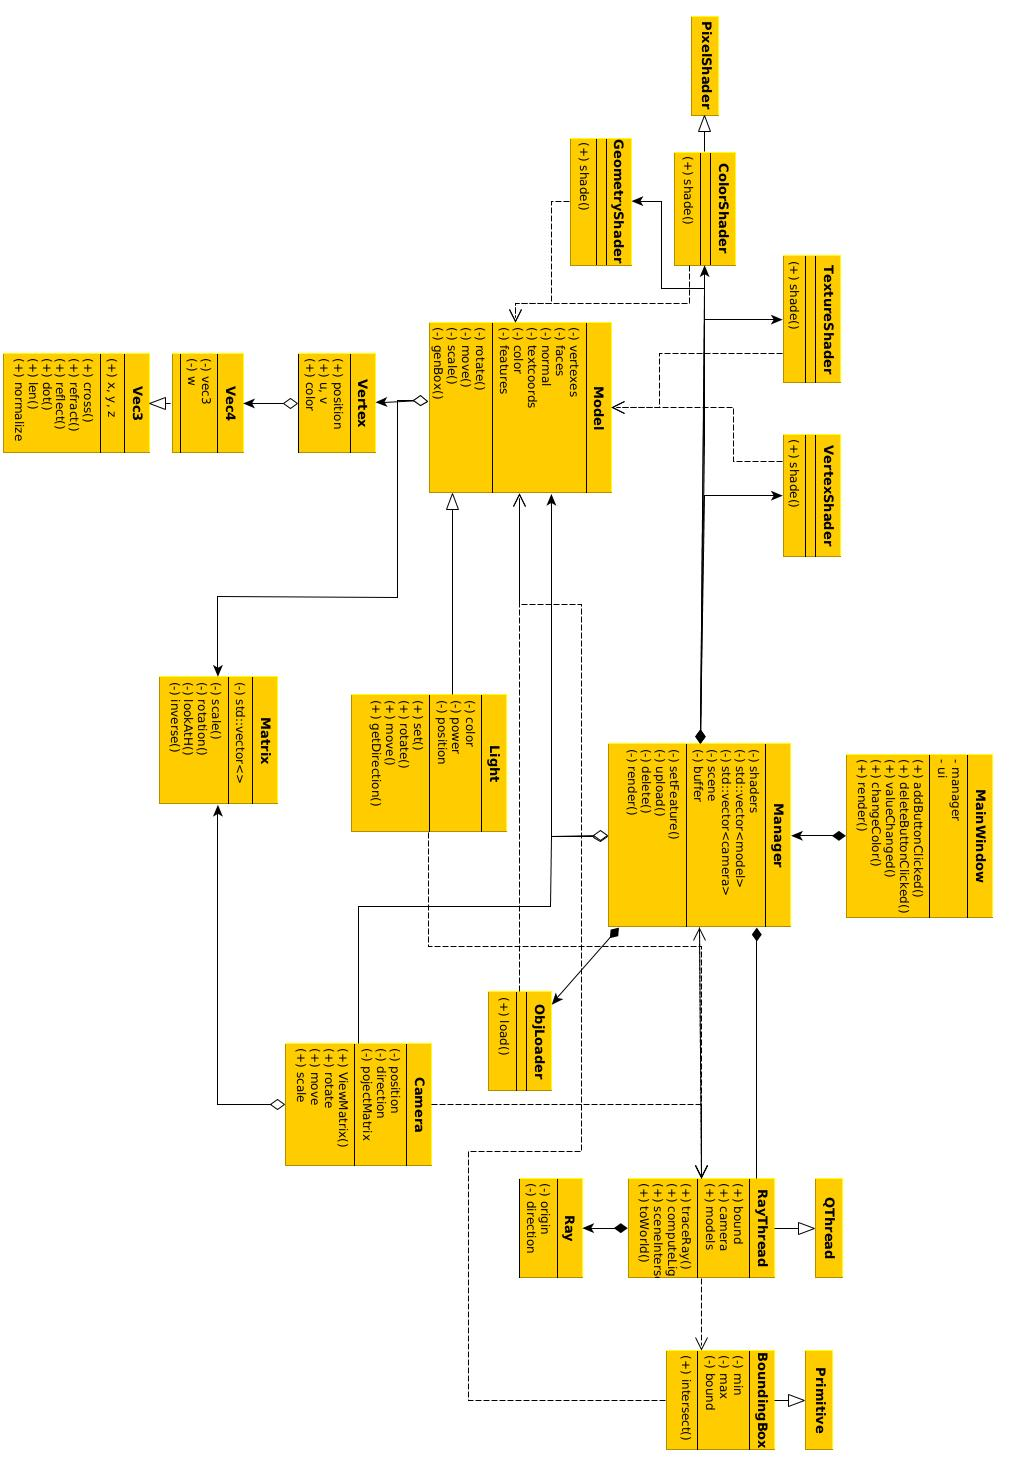
\includegraphics[width=\linewidth]{graph/uml1.jpg}
	\end{center}
	\caption{Диаграмма классов}
\end{figure}
\FloatBarrier

\section{Листинг кода}
На листинге 3.1 представлен код отрисовки модели в первом режиме работы программы:
\FloatBarrier
\begin{lstinputlisting}[language=C++, caption=Код отрисовки модели в первом режиме работы программы, 
	linerange={90-116}, basicstyle=\footnotesize\ttfamily, frame=single,breaklines=true]{src/manager.cpp}
\end{lstinputlisting}
\FloatBarrier

На листинге 3.2 представлен код закраски треугольника в первом режиме работы программы:
\FloatBarrier
\begin{lstinputlisting}[language=C++, caption=Код закраски треугольника в первом режиме работы программы, 
	linerange={120-163}, basicstyle=\footnotesize\ttfamily, frame=single,breaklines=true]{src/manager.cpp}
\end{lstinputlisting}
\FloatBarrier

На листинге 3.3 представлен код алгоритма трассировки одного луча:
\FloatBarrier
\begin{lstinputlisting}[language=C++, caption=Код алгоритма трассировки, 
	linerange={44-115}, basicstyle=\footnotesize\ttfamily, frame=single,breaklines=true]{src/raytraycing.cpp}
\end{lstinputlisting}
\FloatBarrier

На листинге 3.4 представлен код функции поиска пересечения луча с ограничивающим параллелепипедом:

\FloatBarrier
\begin{lstinputlisting}[language=C++, caption=Код отрисовки модели в первом режиме работы программы, 
	linerange={45-74}, basicstyle=\footnotesize\ttfamily, frame=single,breaklines=true]{src/primitive.cpp}
\end{lstinputlisting}
\FloatBarrier

\section{Описание интерфейса}
На рисунке 3.2 представлен стартовый экран программы. 
Он предоставляет пользователю возможность добавить объект, изменить параметры окружающего света и добавления точечного источника.
\FloatBarrier
\begin{figure}[h]
	\begin{center}
		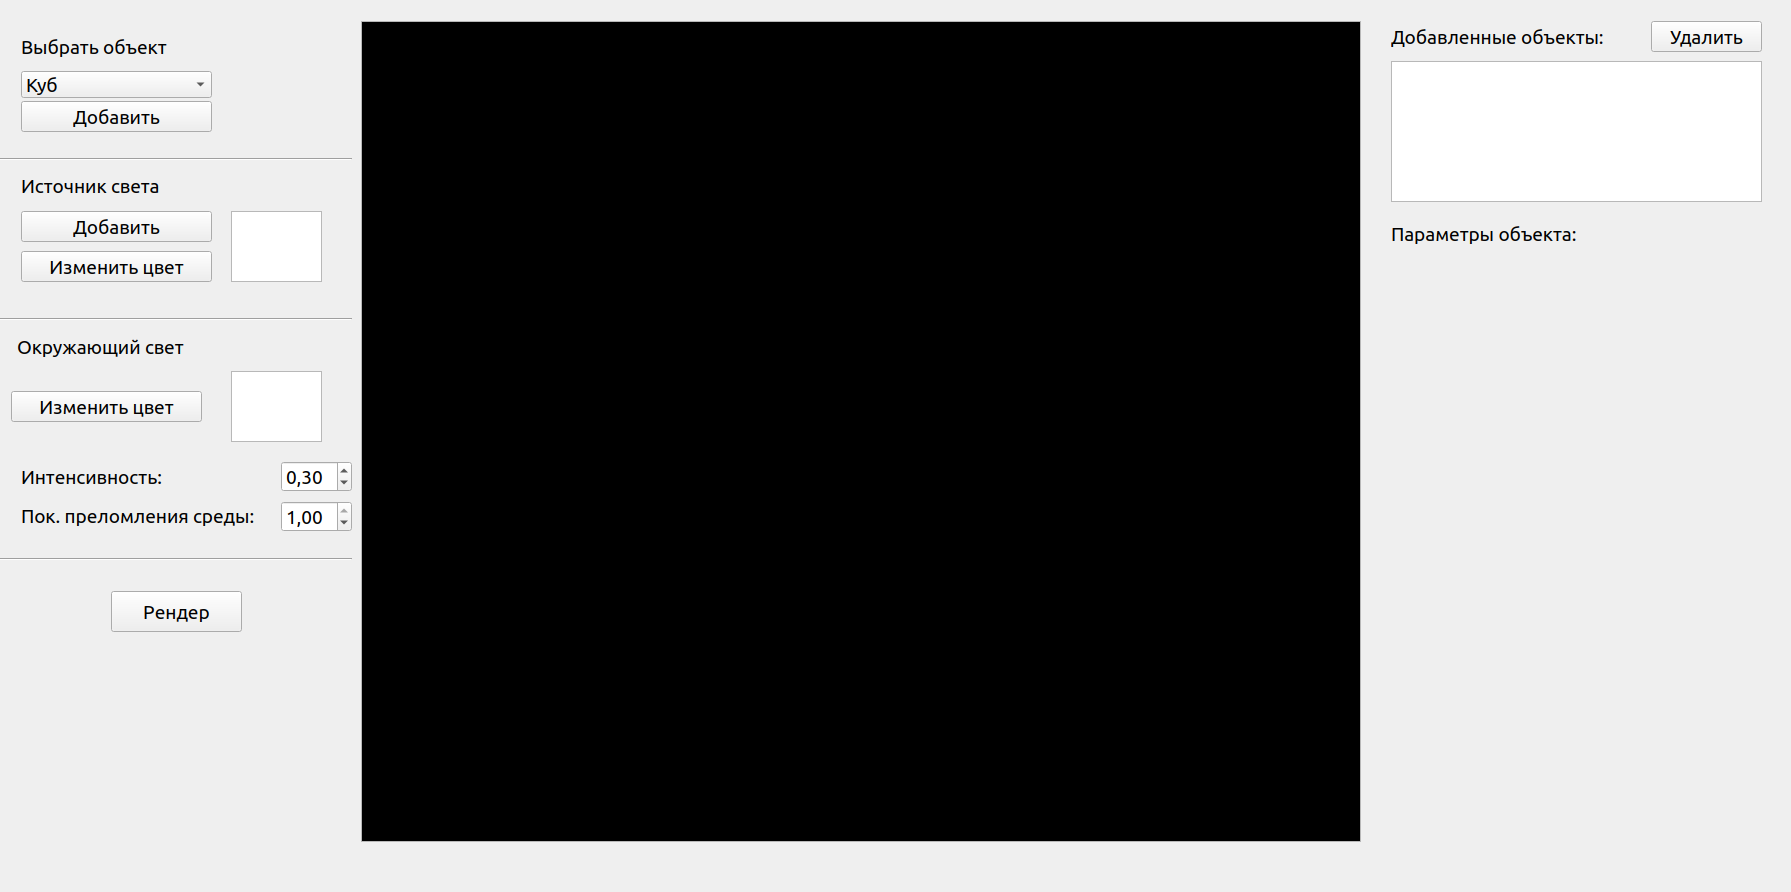
\includegraphics[width=\linewidth]{inc/start.png}
	\end{center}
	\caption{Стартовый экран программы}
\end{figure}
\FloatBarrier

Для добавления объекта модели её нужно выбрать в выпадающем меню в левом верхнем углу, а затем нажать на кнопку добавления.
Модель появится на графике, а также в списке в верхнем правом текстовом поле.

На рисунке 3.3 представлен результат добавления на сцену цилиндра, а также красным подчёркнуты места интерфейса, которые были задействованы:
\FloatBarrier
\begin{figure}[h]
	\begin{center}
		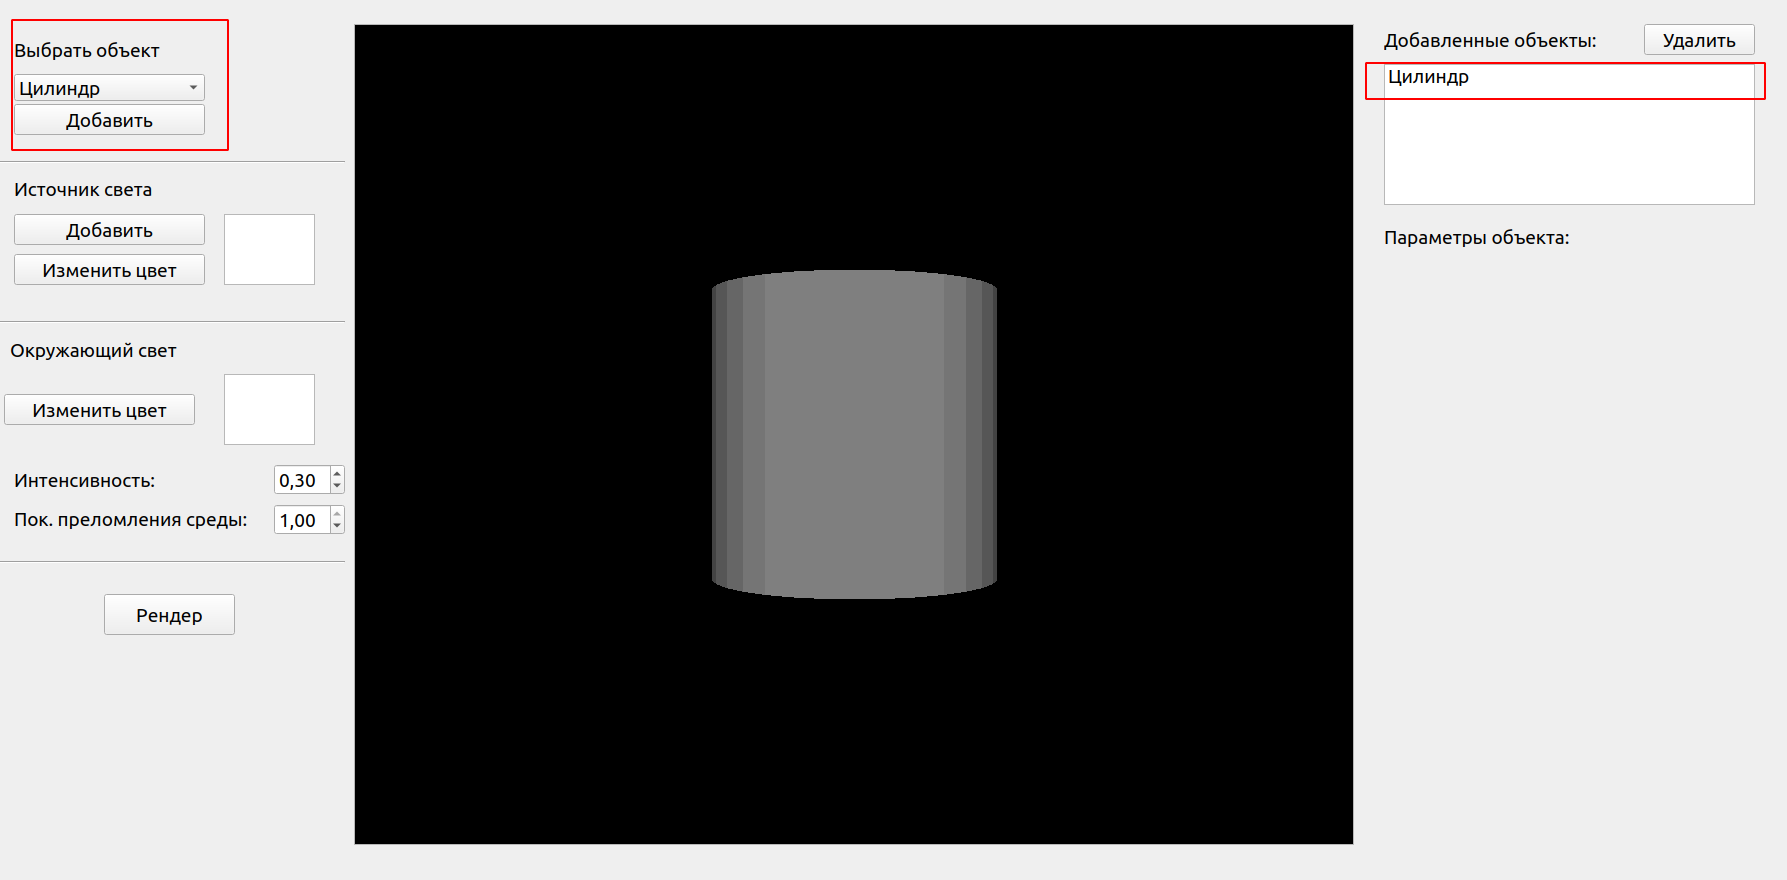
\includegraphics[height = 8cm, width=\linewidth]{inc/add.png}
	\end{center}
	\caption{Экран после добавления на сцену цилиндра}
\end{figure}
\FloatBarrier

При нажатии на название объекта в верхнем правом текстовом поле на экране появляется интерфейс, 
позволяющий изменить параметры модели: пространственное положение, размеры, цвет поверхности или текстуру, физические показатели.

На рисунке 3.4 изображен результат изменения характеристик цилиндра, а также красным подчёркнуты места интерфейса, которые были задействованы:
\FloatBarrier
\begin{figure}[h]
	\begin{center}
		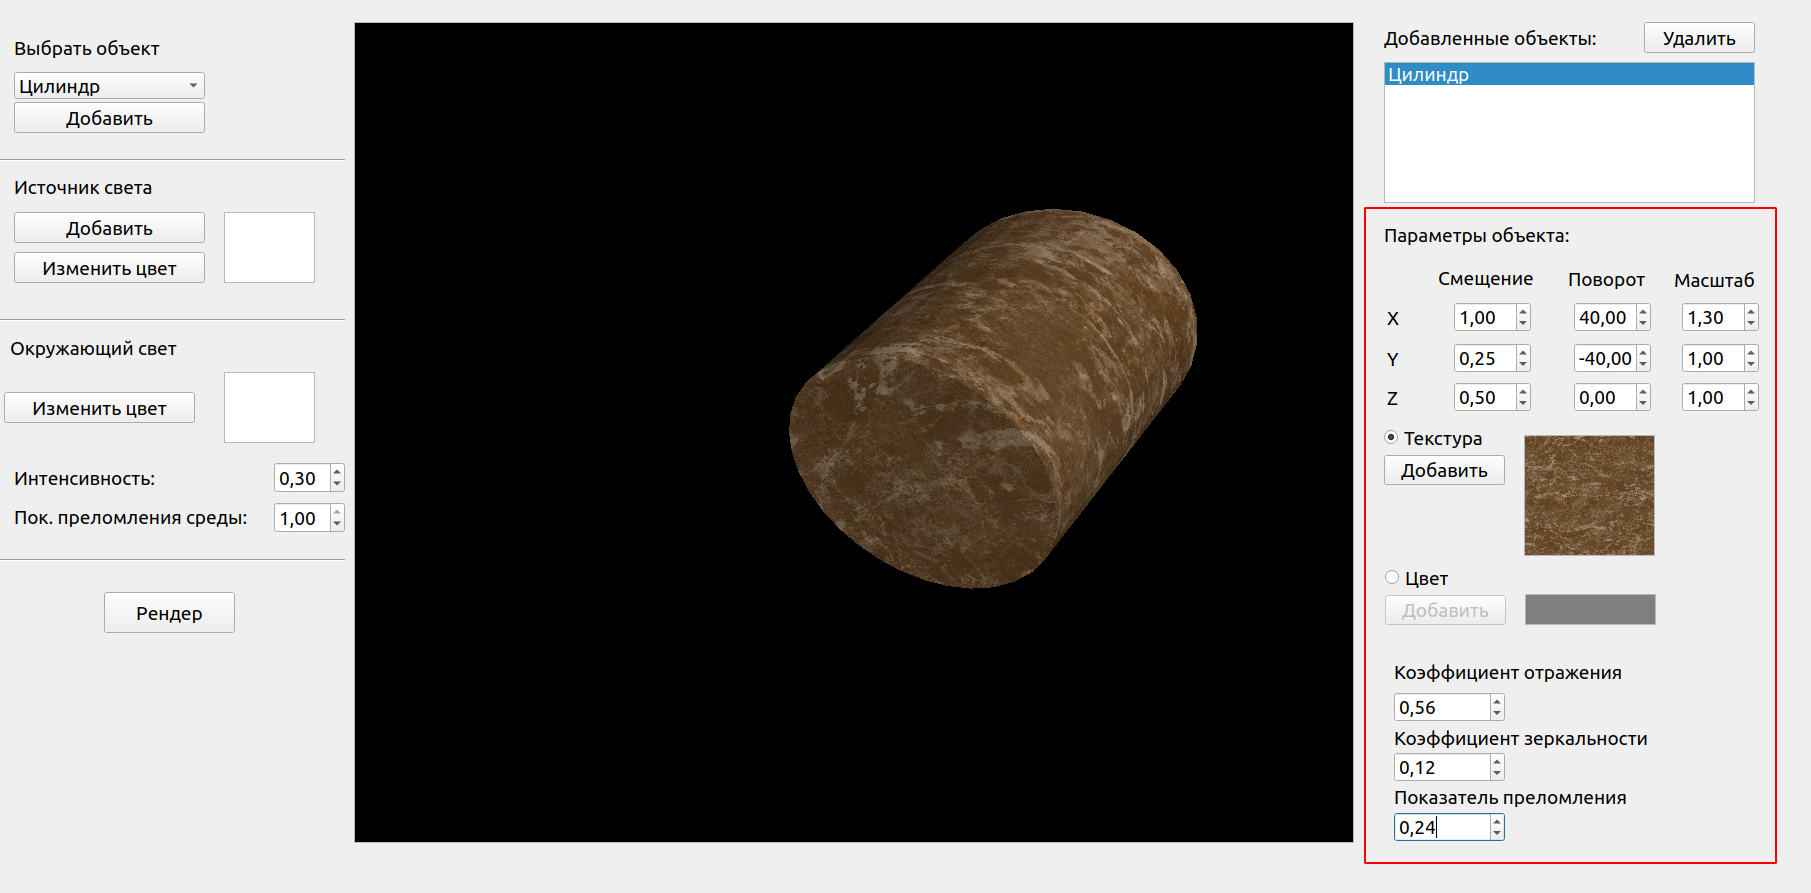
\includegraphics[width=\linewidth]{inc/change.png}
	\end{center}
	\caption{Результат изменения характеристик цилиндра}
\end{figure}
\FloatBarrier

Также слева в поле источника света пользователь может добавить источник света.
После добавления он появится на графике в виде серой точки и в верхнем правом текстовом поле.

На рисунке 3.5 изображен результат добавления источника света на сцену:
\FloatBarrier
\begin{figure}[h]
	\begin{center}
		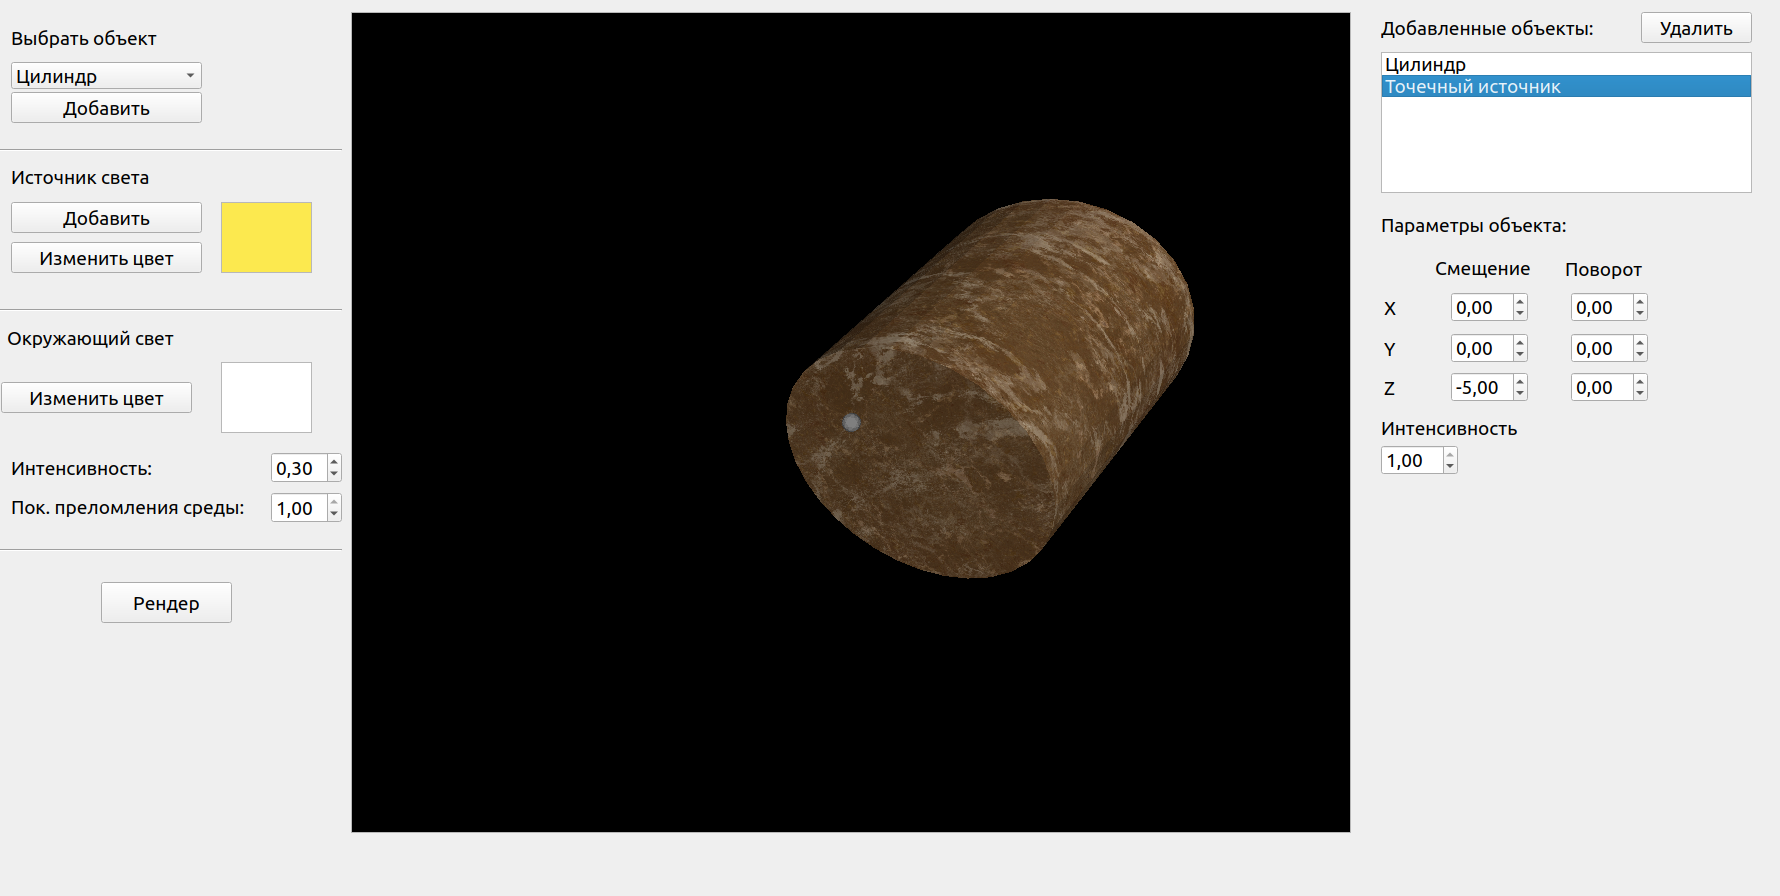
\includegraphics[width=\linewidth]{inc/light.png}
	\end{center}
	\caption{Результат добавления источника света на сцену}
\end{figure}
\FloatBarrier

В поле 'Окружающая среда' пользователь может изменить цвет фонового освещения, его интенсивность, а также изменить показатель преломления среды.
На рисунке 3.6 изображены части интерфейса, которые для этого нужно задействовать.
\FloatBarrier
\begin{figure}[h]
	\begin{center}
		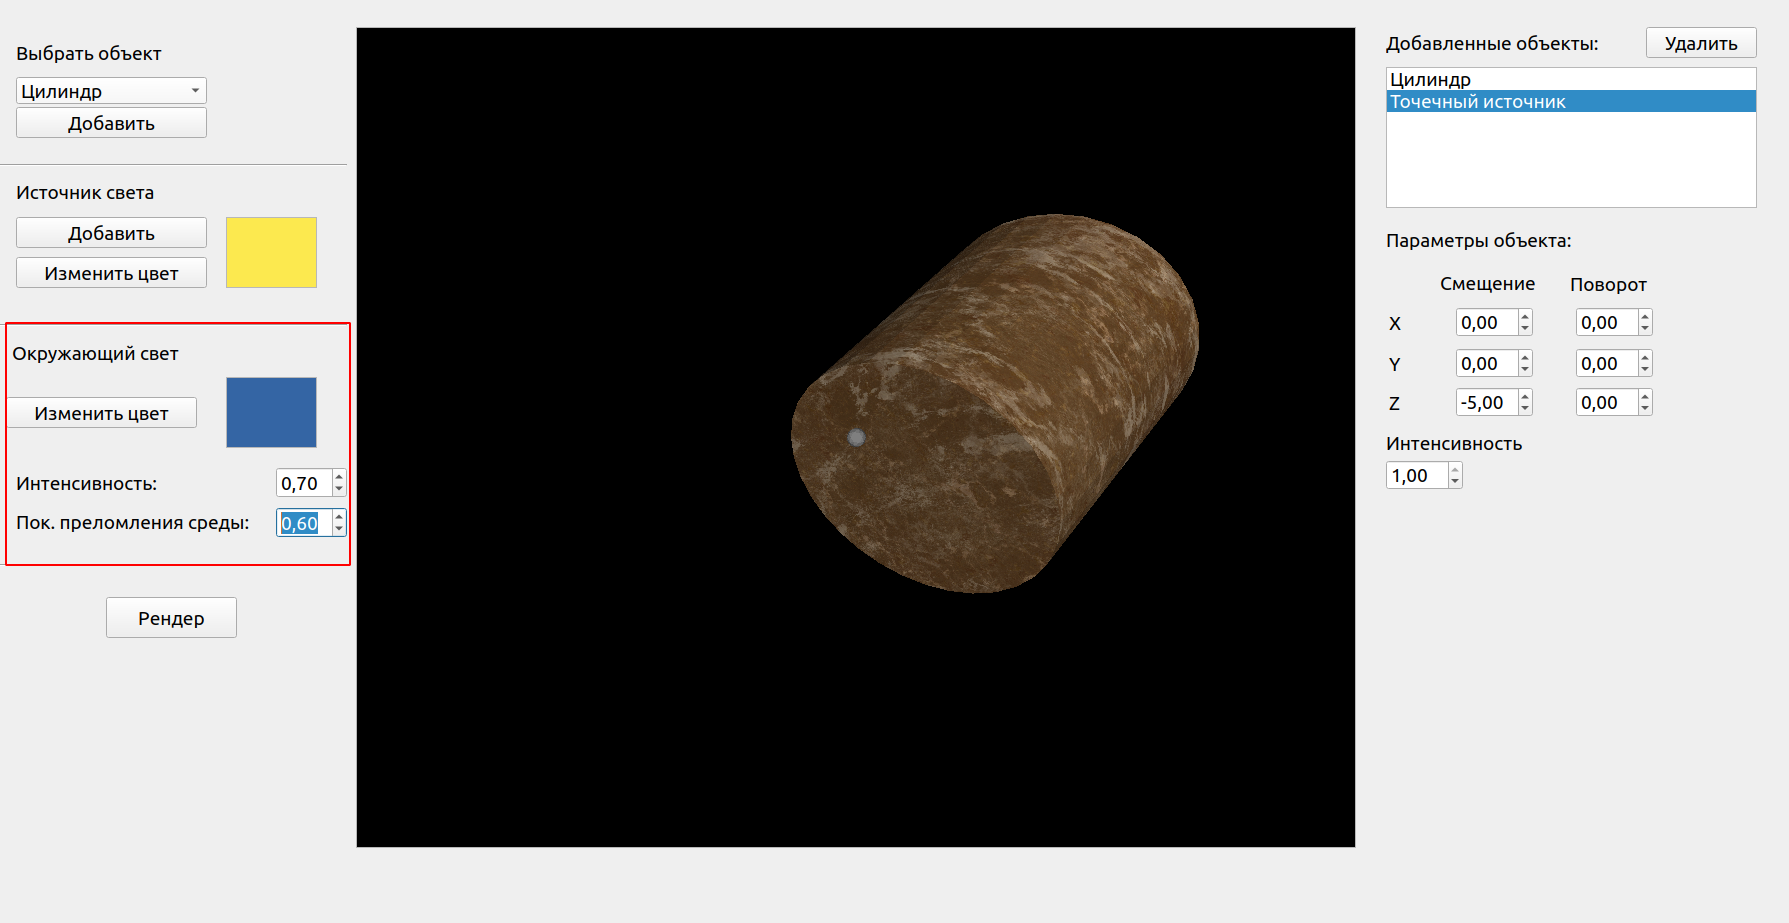
\includegraphics[height = 7cm, width=15cm]{inc/amb.png}
	\end{center}
	\caption{Части интерфейса для изменения параметров окружающей среды}
\end{figure}
\FloatBarrier

При нажатии на кнопку 'Рендер' программа запускает алгоритм обратной трассировки лучей.
Все кнопки блокируются, пока алгоритм не завершит свою работу.
По его окончанию на графике будет отображено реалистическое изображение.
На рисунке 3.7 показано состояние программы в момент рендеринга.
\FloatBarrier
\begin{figure}[h]
	\begin{center}
		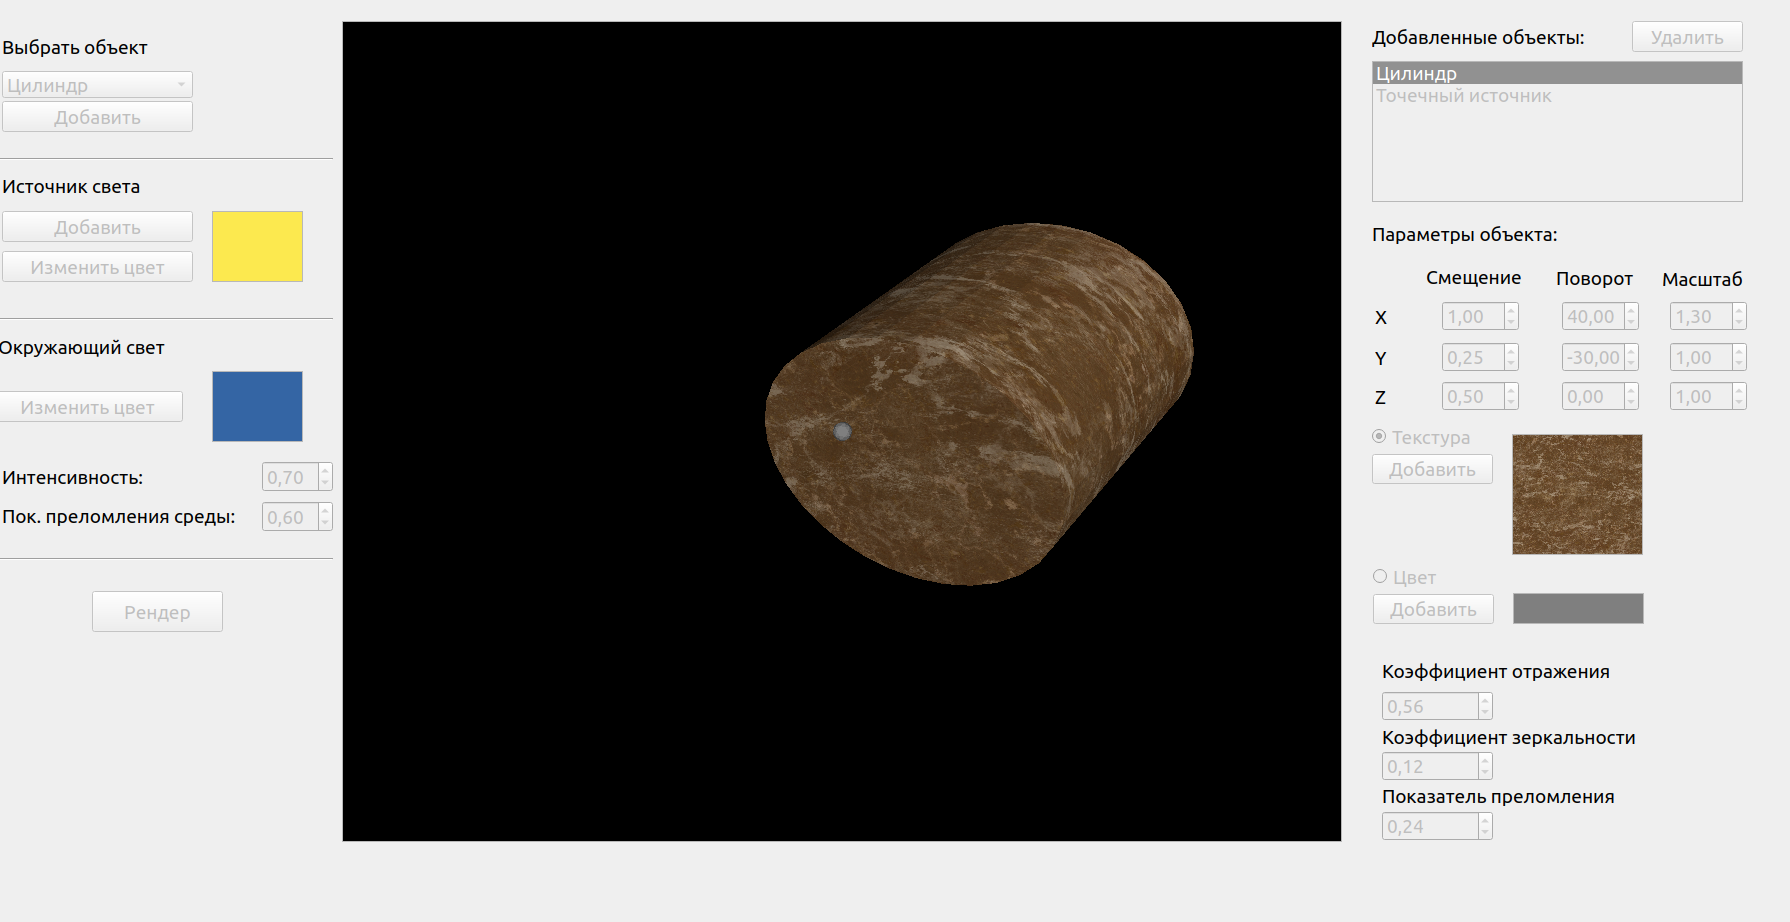
\includegraphics[width=\linewidth]{inc/lock.png}
	\end{center}
	\caption{Процесс рендеринга}
\end{figure}
\FloatBarrier

На рисунке 3.8 показан конечный результат работы алгоритма обратной трассировки лучей.
\FloatBarrier
\begin{figure}[h]
	\begin{center}
		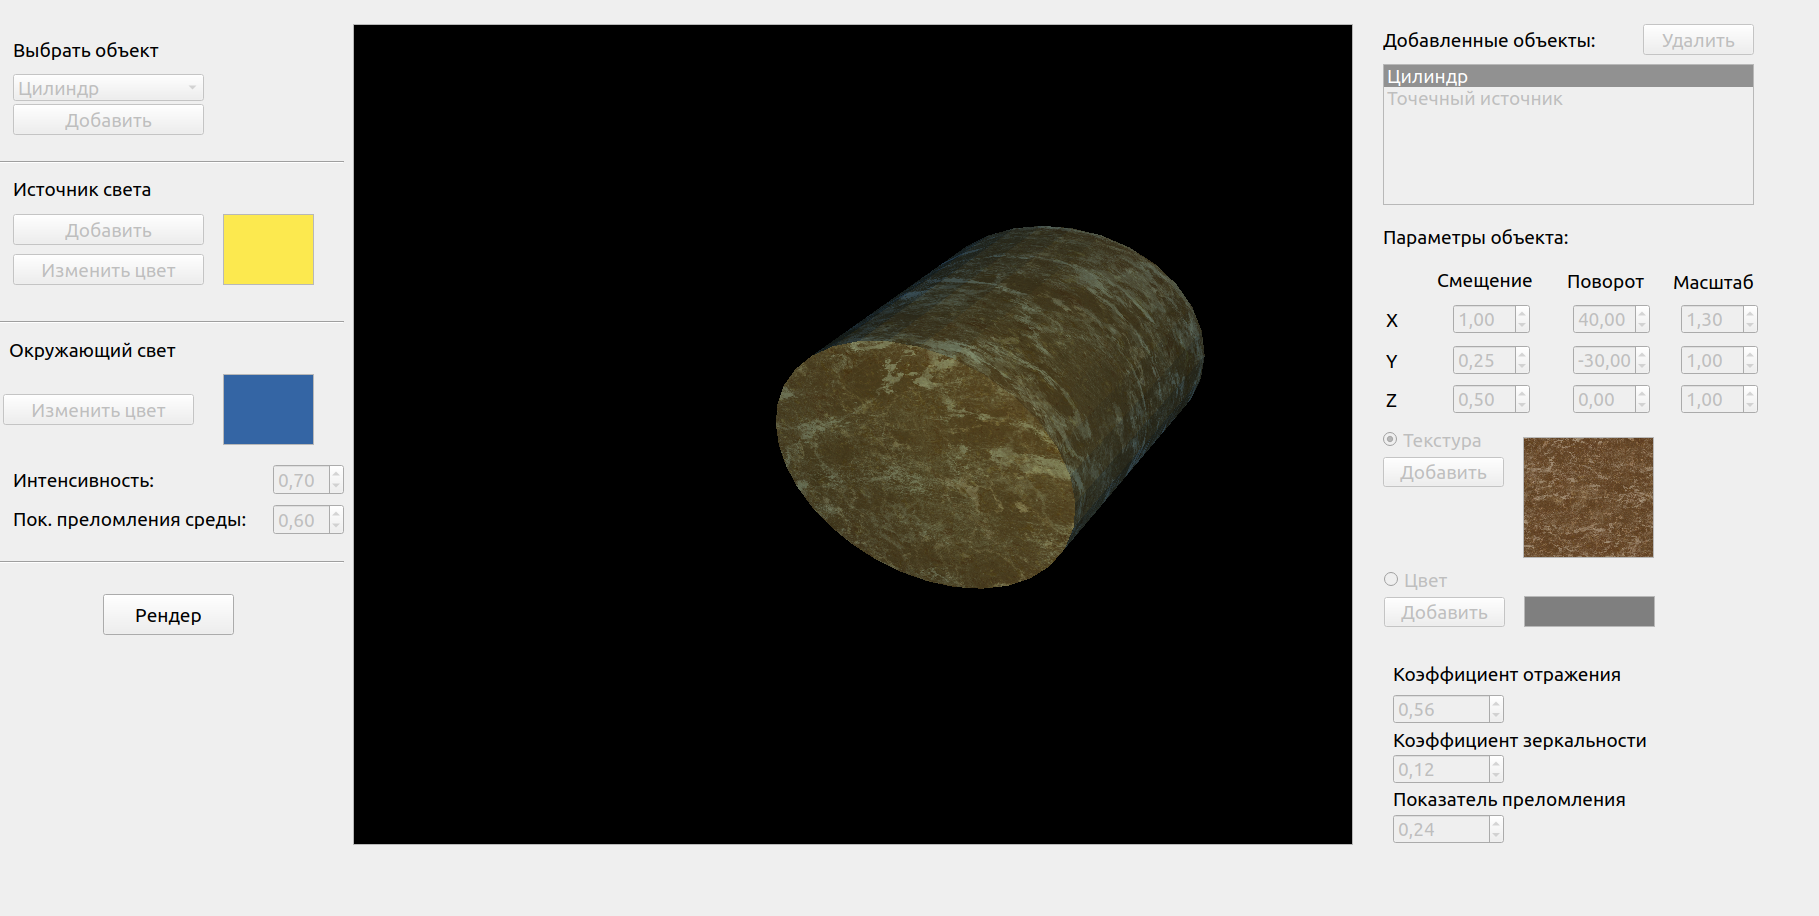
\includegraphics[height = 7cm, width=15cm]{inc/result.png}
	\end{center}
	\caption{Результат работы программы}
\end{figure}
\FloatBarrier

Для того, чтобы вернуться к редактированию изображению, пользователь может нажать на кнопку 'Рендер'.
Управление камерой осуществляется при помощи клавиатуры кнопками W, E, S, D, X, Home, End, PageUp, PageDown. 

\section{Вывод}
Было приведено описание структура программы, выбраны средства реализации ПО,
приведены листинги кода, и продемонстрирован интерфейс программы.